\begin{frame}{总结：从线性响应到超快非平衡动力学}

  \small
  \setlength{\abovedisplayskip}{2pt}
  \setlength{\belowdisplayskip}{2pt}

  {\scriptsize\color{gray}JCP 2024\par}
  \[
    \text{强耦合 cavity--molecule system}
    \longrightarrow\chi(\omega)
    \longrightarrow T(\omega),\,R(\omega),\,A(\omega)
  \]
  {\centering\scriptsize
    弱 probe 读取已形成的 LP/UP 线性共振。\par}

  \vspace{0.3em}
  \[
    \text{pump 将体系推离平衡}
    \quad\Longrightarrow\quad
    \rho(t)\ \longleftrightarrow\ \alpha(t)
  \]
  {\centering\scriptsize
    分子态与腔场必须自洽实时演化，$P(t)=\Tr[\hat\mu\rho(t)]$。\par}

  \vspace{0.3em}
  {\scriptsize\color{gray}PRL 2025\par}
  \[
    p^2p'
    \longrightarrow\alpha^{(2)(1)}
    \longrightarrow\Delta T(\omega,\tau_\Delta)
  \]
  {\centering\scriptsize
    相干：早时间振荡\qquad 布居：长时间谱修正。\par}

  \vspace{0.4em}
  {\centering\small
    第二篇在一阶弱场极限恢复第一篇的线性极化激元响应。\par}

\end{frame}

\begin{frame}{数值图复现与核验}

  \setlength{\abovedisplayskip}{2pt}
  \setlength{\belowdisplayskip}{2pt}

  \begin{columns}[c,onlytextwidth]
    \begin{column}{0.48\textwidth}
      {\centering
        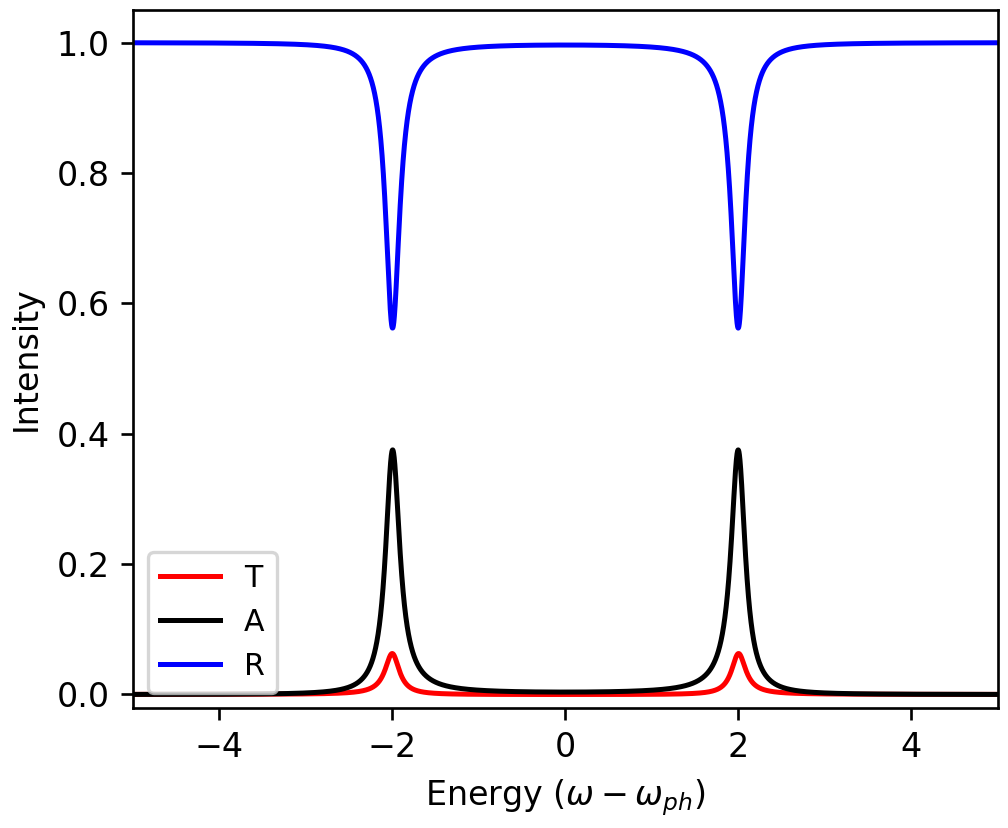
\includegraphics[height=0.41\textheight,keepaspectratio]
          {../figures/linear/fig3a_reproduction.png}\par}
      {\centering\tiny\color{gray}JCP Fig.~3(a)\par}
    \end{column}
    \begin{column}{0.48\textwidth}
      {\centering
        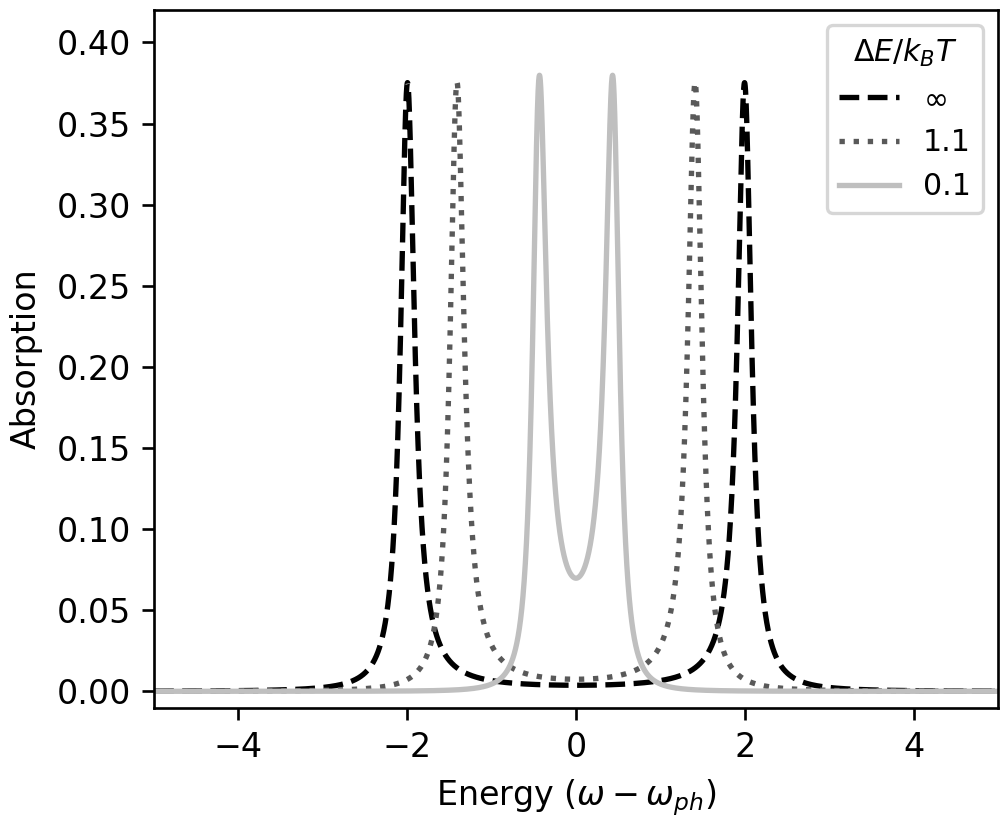
\includegraphics[height=0.41\textheight,keepaspectratio]
          {../figures/linear/fig3b_reproduction.png}\par}
      {\centering\tiny\color{gray}JCP Fig.~3(b)\par}
    \end{column}
  \end{columns}

  \vspace{0.3em}

  \begin{columns}[c,onlytextwidth]
    \begin{column}{0.48\textwidth}
      {\centering
        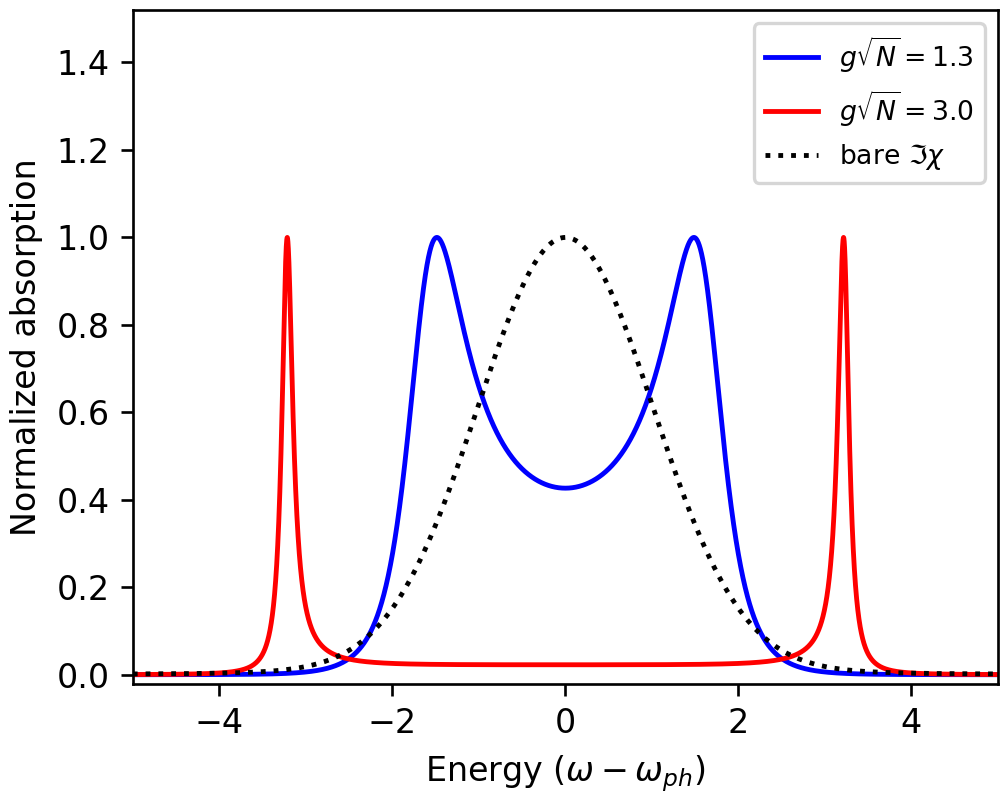
\includegraphics[height=0.41\textheight,keepaspectratio]
          {../figures/linear/fig4c_reproduction.png}\par}
      {\centering\tiny\color{gray}JCP Fig.~4(c)\par}
    \end{column}
    \begin{column}{0.48\textwidth}
      {\centering
        
\includegraphics[height=0.41\textheight,keepaspectratio]
          {../figures/nonlinear/fig3_reproduction.png}\par}
      {\centering\tiny\color{gray}PRL Fig.~3\par}
    \end{column}
  \end{columns}

  \vspace{0.25em}

  {\centering\tiny\color{gray}
    Codex（GPT-5.6 Sol）一次完整复现工作流运行约 47 min，
    已有复现结果与原文基本一致。\par}

\end{frame}

\backmatter

\begin{frame}{二能级分子线性极化率}

  \small
  \setlength{\abovedisplayskip}{3pt}
  \setlength{\belowdisplayskip}{3pt}

  {\footnotesize\textbf{1. 一阶光学相干运动方程}}
  \[
    \dot\rho_{eg}^{(1)}
    =-\left(\ii\omega_0+\frac{\gamma}{2}\right)\rho_{eg}^{(1)}
    +\ii\frac{\mu_{eg}}{\hbar}(p_g-p_e)E(t).
  \]

  \vspace{0.4em}
  {\footnotesize\textbf{2. 单频驱动下的频域解}}
  \[
    \rho_{eg}^{(1)}(\omega)
    =-\frac{\mu_{eg}}{\hbar}
    \frac{p_g-p_e}{\omega-\omega_0+\ii\gamma/2}E(\omega).
  \]

  \vspace{0.4em}
  {\footnotesize\textbf{3. 第一篇腔耦合归一化后的极化率}}
  \vspace{1.5em}
  \[
    \chi_{\mathrm{2LS}}(\omega)
    =-\frac{
      \physmark{Plum}{p26G2}{G^2}
      \physmark{Bittersweet}{p26pgpe}{(p_g-p_e)}
    }{\omega-\physmark{NavyBlue}{p26w0}{\omega_0}
      +\ii\physmark{OliveGreen}{p26gam}{\gamma/2}}
  \]
  \begin{tikzpicture}[overlay,remember picture,>=stealth,
      nodes={align=center,inner ysep=1pt},<-]
    \path (p26G2.south) ++ (-0.9,3.8em)
      node[anchor=north,color=Plum!85] (p26G2text)
      {\textsf{\footnotesize 集体耦合权重}};
    \draw[color=Plum] (p26G2.north) |- (p26G2text.south);
    \path (p26pgpe.south) ++ (1.2,3.8em)
      node[anchor=north,color=Bittersweet!85] (p26pgpetext)
      {\textsf{\footnotesize 布居差 / 净响应权重}};
    \draw[color=Bittersweet] (p26pgpe.north) |- (p26pgpetext.south);
    \path (p26w0.south) ++ (-0.75,-0.8em)
      node[anchor=north,color=NavyBlue!85] (p26w0text)
      {\textsf{\footnotesize 共振位置}};
    \draw[color=NavyBlue] (p26w0.south) |- (p26w0text.north);
    \path (p26gam.south) ++ (1.5,-2.0em)
      node[anchor=north,color=OliveGreen!85] (p26gamtext)
      {\textsf{\footnotesize 光学相干线宽}};
    \draw[color=OliveGreen] (p26gam.south) |- (p26gamtext.north);
  \end{tikzpicture}
  \vspace{2.2em}

\end{frame}

\begin{frame}{标准腔输入--输出关系}

  \footnotesize
  \setlength{\abovedisplayskip}{2pt}
  \setlength{\belowdisplayskip}{2pt}

  \begin{columns}[c,onlytextwidth]
    \begin{column}{0.30\textwidth}
      {\centering
        \begin{tikzpicture}[>=stealth,x=0.8cm,y=0.8cm,
            every node/.style={inner sep=2pt,font=\scriptsize}]
          \draw[line width=1.3pt] (1.1,-1.3) -- (1.1,1.3);
          \draw[line width=1.3pt] (2.4,-1.3) -- (2.4,1.3);
          \node at (1.1,1.65) {$\kappa_L$};
          \node at (2.4,1.65) {$\kappa_R$};
          \node[text=Plum,font=\large] at (1.75,0) {$a$};
          \draw[->,NavyBlue,thick] (-0.6,0.55) -- (1.02,0.55);
          \node[text=NavyBlue] at (0.1,1.02) {$a_{\mathrm{in,L}}$};
          \draw[->,OliveGreen,thick] (1.02,-0.55) -- (-0.6,-0.55);
          \node[text=OliveGreen] at (0.1,-1.02) {$a_{\mathrm{out,L}}$};
          \draw[->,OliveGreen,thick] (2.48,0) -- (4.1,0);
          \node[text=OliveGreen] at (3.55,0.5) {$a_{\mathrm{out,R}}$};
        \end{tikzpicture}\par}
      {\centering $\kappa=\kappa_L+\kappa_R$。\par}
      \vspace{0.5em}
      {\fontsize{7}{8.5}\selectfont\color{gray}
        相干振幅；$a_{\mathrm{in,R}}=0$。\par
        $\omega_c\equiv\omega_{\mathrm{ph}}$（p\pageref{frame:cavity-response}）。\par
        单频 $e^{-\ii\omega t}$；旋波、马尔可夫近似。
      }
    \end{column}
    \begin{column}{0.67\textwidth}
      \[
        \dot a=-\left(\ii\omega_c+\tfrac\kappa2\right)a
          +\sqrt{\kappa_L}\,a_{\mathrm{in,L}}+\mathcal F_{\mathrm{mol}}.
      \]
      {\scriptsize\color{gray}
        线性分子反馈：$\mathcal F_{\mathrm{mol}}(\omega)=\ii\chi(\omega)a(\omega)$。
      }
      \[
        \begin{aligned}
          a(\omega)&=\ii\sqrt{\kappa_L}\,D^R(\omega)a_{\mathrm{in,L}}(\omega),\\
          D^R(\omega)&=\frac{1}{\omega-\omega_c+\ii\kappa/2+\chi(\omega)}.
        \end{aligned}
      \]
      \[
        a_{\mathrm{out,L}}=a_{\mathrm{in,L}}-\sqrt{\kappa_L}\,a,
        \qquad a_{\mathrm{out,R}}=-\sqrt{\kappa_R}\,a.
      \]
      {\scriptsize
        振幅比：$r=a_{\mathrm{out,L}}/a_{\mathrm{in,L}}$，
        $t=a_{\mathrm{out,R}}/a_{\mathrm{in,L}}$。
      }
      \[
        r(\omega)=1-\ii\kappa_LD^R(\omega),
        \qquad t(\omega)=-\ii\sqrt{\kappa_L\kappa_R}\,D^R(\omega).
      \]
      \[
        T=|t|^2,\qquad R=|r|^2,\qquad A=1-T-R.
      \]
    \end{column}
  \end{columns}

  \vspace{0.4em}
  \[
    T(\omega)=\frac{\kappa_L\kappa_R}
      {|\omega-\omega_c+\ii\kappa/2+\chi(\omega)|^2},
    \qquad
    A(\omega)=\frac{2\kappa_L\operatorname{Im}\chi(\omega)}
      {|\omega-\omega_c+\ii\kappa/2+\chi(\omega)|^2}.
  \]

  {\fontsize{6.3}{7.4}\selectfont\color{gray}
    PRL 保留自身输入归一化；本页端口场取相反整体相位，
    $\sqrt{\kappa_L}a_{\mathrm{in,L}}=-\eta f(t)e^{-\ii\omega_l t}$。
  }
  \papersource{JCP 160, 154107 (2024), Eqs.~(27), (32)--(34), (A9), (A13), (B9); PRL SM S2.}

\end{frame}
